% All measurements and organizational claims in this deck are synthetic.
\documentclass[11pt,aspectratio=169]{beamer}
\usetheme[listings]{Tempus}
\usepackage{booktabs}
\usepackage[authoryear,round]{natbib}
% The enclosing frame supplies the heading; avoid an extra bibliography section.
\renewcommand{\bibsection}{}
\usetikzlibrary{arrows.meta,positioning}
\title[From pilot to practice]{From pilot to practice}
\subtitle{Technical evidence and an executive decision}
\author{Alex Morgan \and Sam Rivera}
\institute{Tempus Research Lab}
\date{October 2026}
\titlegraphic{\tempusartwork{examples/assets/mark}}
\begin{document}
\begin{frame}[plain]
  \titlepage
\end{frame}
\begin{frame}{Agenda}
  \tableofcontents
  \bigskip
  \textcolor{TempusMuted}{A synthetic pilot: evidence, tradeoffs, and a bounded next step.}
\end{frame}
\section{Decision context}
\begin{frame}[plain]
  \reportlogomark\par\bigskip
  {\usebeamerfont{title}\textcolor{TempusAccent}{01 / Decision context}}\par
  \medskip What must be true before expanding the pilot?
\end{frame}
\begin{frame}{A smaller pilot can answer the largest uncertainty}
  \begin{itemize}[<+->]
    \item The team needs reliable predictions within a fixed latency budget.
    \item A controlled pilot separates model quality from workflow effects.
    \item Expansion depends on both technical and operational evidence.
  \end{itemize}
  \begin{block}{Note: scope of the evidence}
    All results here are synthetic; they illustrate a presentation structure.
  \end{block}
\end{frame}
\begin{frame}{Compare alternatives against the same constraints}
  \begin{columns}[T,onlytextwidth]
    \begin{column}{.47\textwidth}
      \begin{block}{Option A / baseline}
        Lower integration effort.\par\medskip
        Predictable operating cost.\par\medskip
        Smaller quality improvement.
      \end{block}
    \end{column}
    \begin{column}{.47\textwidth}
      \begin{exampleblock}{Option B / encoder}
        Better pilot accuracy.\par\medskip
        Additional monitoring work.\par\medskip
        Fits the latency budget.
      \end{exampleblock}
    \end{column}
  \end{columns}
  \medskip\textbf{Shared conclusion:} test Option B in a bounded deployment.
\end{frame}
\section{Technical evidence}
\begin{frame}{The workflow makes each transformation inspectable}
  \centering
  \begin{tikzpicture}[node distance=5mm,
    stage/.style={draw=TempusRule,fill=TempusLight,minimum width=23mm,
      minimum height=12mm,align=center,font=\sffamily\small},
    flow/.style={-{Stealth},draw=TempusAccent}]
    \node[stage] (data) {Input\\batch};
    \node[stage,right=of data] (encoder) {Compact\\encoder};
    \node[stage,right=of encoder] (score) {Class\\scores};
    \node[stage,right=of score] (review) {Human\\review};
    \draw[flow] (data)--(encoder);
    \draw[flow] (encoder)--(score);
    \draw[flow] (score)--(review);
  \end{tikzpicture}\par\medskip
  \raggedright\small Source: original editable TikZ diagram; synthetic workflow.
  \begin{exampleblock}{Tip: retain observability}
    Record latency and review outcomes at each boundary.
  \end{exampleblock}
\end{frame}
\begin{frame}{A simple loss connects predictions to labels}
  For batch size $B$ and class count $C$, minimize cross-entropy:
  \begin{equation}
    \mathcal{L}=-\frac{1}{B}\sum_{i=1}^{B}\sum_{c=1}^{C}
      y_{ic}\log p_{ic}.
    \label{eq:deck-loss}
  \end{equation}
  Attention-based representations motivate the encoder
  \citep{vaswani2017attention}.
  \begin{alertblock}{Warning: validation is separate from training}
    Select operating thresholds on held-out data, then test once.
  \end{alertblock}
\end{frame}
\begin{frame}{Quality improves within the pilot latency budget}
  \begin{columns}[T,onlytextwidth]
    \begin{column}{.48\textwidth}
      \small
      \begin{tabular}{lrr}
        \toprule
        Model & Accuracy & Latency\\
        \midrule
        Baseline & 81\% & 12 ms\\
        Encoder & 87\% & 18 ms\\
        \bottomrule
      \end{tabular}\par\medskip
      \textbf{Interpretation:} +6 percentage points at +6 ms.
    \end{column}
    \begin{column}{.46\textwidth}
      \centering
      \begin{tikzpicture}[x=.07\linewidth,y=.035\linewidth]
        \draw[TempusRule] (0,0)--(10,0);
        \fill[TempusSage] (1,0) rectangle (4,8.1);
        \fill[TempusTeal] (6,0) rectangle (9,8.7);
        \node[font=\sffamily\small,above] at (2.5,8.1) {81\%};
        \node[font=\sffamily\small,above] at (7.5,8.7) {87\%};
        \node[font=\sffamily\fontsize{8}{9}\selectfont,below] at (2.5,0) {Baseline};
        \node[font=\sffamily\fontsize{8}{9}\selectfont,below] at (7.5,0) {Encoder};
      \end{tikzpicture}
    \end{column}
  \end{columns}
  \medskip\small Source: synthetic held-out pilot, $n=1{,}000$;
  accuracy bars start at zero. See equation~\ref{eq:deck-loss}.
\end{frame}
\begin{frame}{Use images with a descriptive source and clear purpose}
  \begin{columns}[c,onlytextwidth]
    \begin{column}{.30\textwidth}
      \centering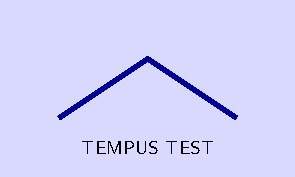
\includegraphics[width=25mm,height=25mm,keepaspectratio]{examples/assets/mark.pdf}
    \end{column}
    \begin{column}{.65\textwidth}
      The shared T mark combines a navy crossbar and stem with a teal time tick.
      \par\medskip\small Source: bundled vector artwork, exported from
      \texttt{\string\reportlogomark}; original Tempus design.
    \end{column}
  \end{columns}
\end{frame}
\begin{frame}[fragile]{Keep implementation examples short and readable}
  \begin{lstlisting}[language=Python]
def accept_candidate(accuracy, latency_ms):
    # Synthetic operating gates.
    quality_ok = accuracy >= 0.85
    latency_ok = latency_ms <= 20
    return quality_ok and latency_ok
  \end{lstlisting}
  \begin{block}{Note: code is optional}
    Enable the theme's listings option and use a fragile frame.
    Split long examples across frames; the default code size is 8 pt.
  \end{block}
\end{frame}
\section{Executive recommendation}
\begin{frame}{Three metrics describe the pilot, not the whole system}
  \begin{columns}[T,onlytextwidth]
    \begin{column}{.30\textwidth}
      \begin{block}{Quality}
        {\sffamily\Large\textcolor{TempusAccent}{87\%}}\par
        Accuracy\par\small Held-out sample\par $n=1{,}000$
      \end{block}
    \end{column}
    \begin{column}{.30\textwidth}
      \begin{exampleblock}{Speed}
        {\sffamily\Large\textcolor{TempusTeal}{18 ms}}\par
        Median latency\par\small Single request\par CPU inference
      \end{exampleblock}
    \end{column}
    \begin{column}{.30\textwidth}
      \begin{alertblock}{Effort}
        {\sffamily\Large\textcolor{TempusAmber}{2 weeks}}\par
        Pilot duration\par\small Two engineers\par Fixed scope
      \end{alertblock}
    \end{column}
  \end{columns}
  \medskip\small Context: synthetic planning figures; no production guarantee.
\end{frame}
\begin{frame}{Four milestones keep expansion reversible}
  \begin{enumerate}
    \item \textcolor{TempusAccent}{Week 1 / Prepare}: freeze data and success criteria.
    \item \textcolor{TempusTeal}{Week 2 / Evaluate}: verify quality and latency.
    \item \textcolor{TempusAmber}{Week 3 / Pilot}: monitor a limited user cohort.
    \item \textcolor{TempusBurgundy}{Week 4 / Decide}: expand, revise, or stop.
  \end{enumerate}
  \medskip\textcolor{TempusMuted}{Each milestone has an owner and a recorded decision.}
\end{frame}
\begin{frame}{Approve a bounded pilot with explicit stopping criteria}
  \begin{importantblock}{Important: decision requested}
    Approve a two-week pilot of the compact encoder.
  \end{importantblock}
  \textbf{Evidence:} quality improves by six percentage points while
  median latency stays below 20 ms.\par\medskip
  \textbf{Next step:} assign an owner and review drift, latency, and user outcomes
  before expanding the cohort.
\end{frame}
\begin{frame}{References}
  \bibliographystyle{acl_natbib}
  \bibliography{reference}
\end{frame}
\begin{frame}[plain]
  \reportlogomark\par\bigskip
  {\usebeamerfont{title}\textcolor{TempusAccent}{A decision grounded in evidence}}\par
  \medskip Questions and discussion\par\medskip
  \href{mailto:research@example.org}{research@example.org}
\end{frame}
\end{document}
